\section{DESIGN APPROACH}

   \begin{figure}[thpb]
      \centering
      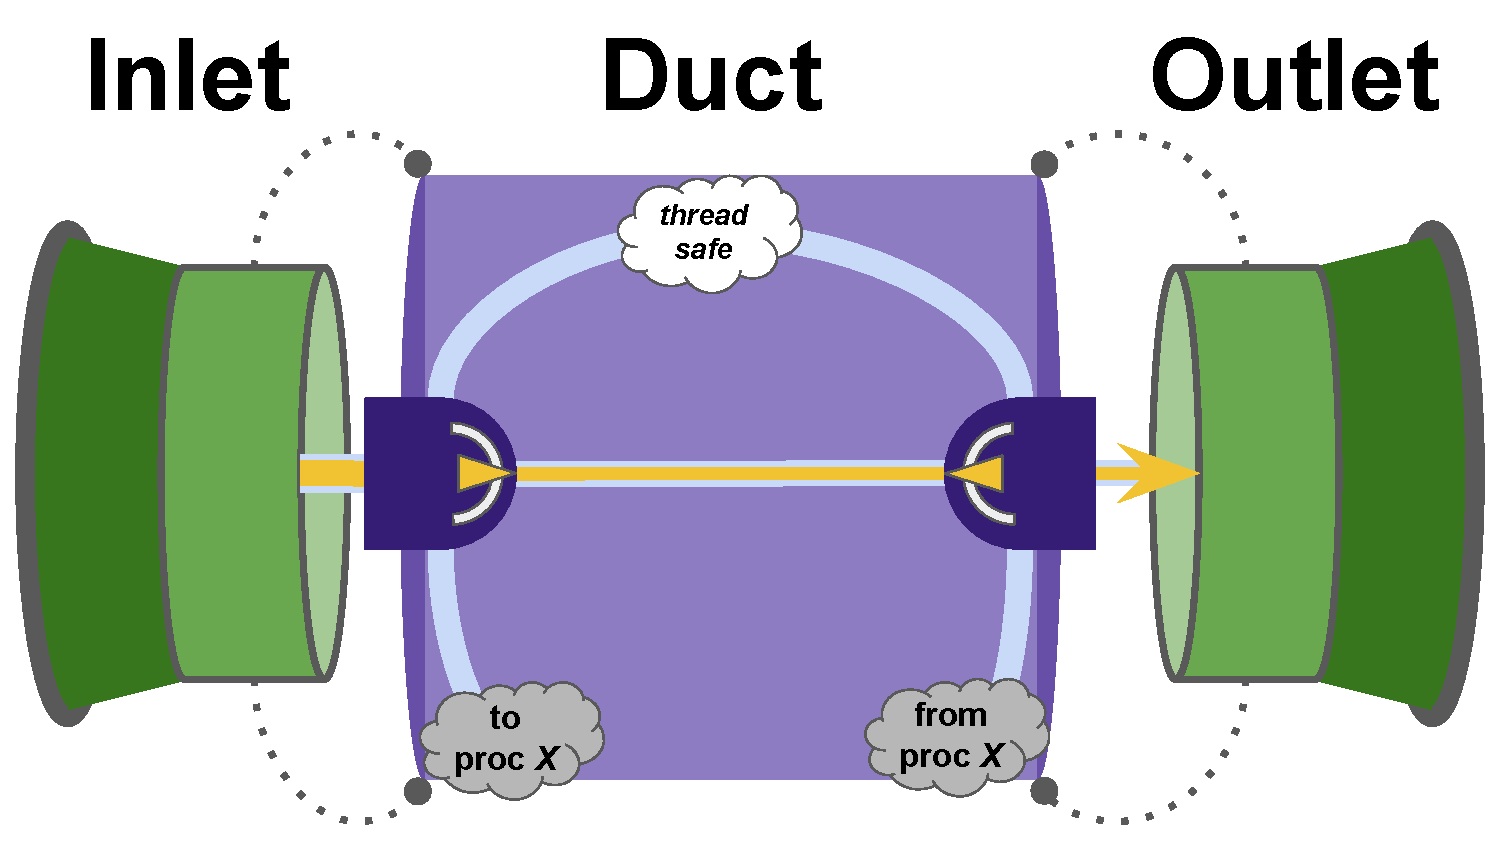
\includegraphics[width=0.8\linewidth]{img/conduit}
      \caption{Schematic of Conduit's \texttt{Inlet} and \texttt{Outlet} object scheme, where communication behavior is controlled, invisibly to the end-user, by an underlying \texttt{Duct} object.}
      \label{fig:conduit}
   \end{figure}

Conduit represents communication in terms of a paired \texttt{Inlet}, which accepts messages, and \texttt{Outlet}, which dispenses messages.
An \texttt{Inlet} and \texttt{Outlet} may exchange messages via an intra-thread, inter-thread, or inter-process communication procedure, depending on the runtime state of an underlying held \texttt{Duct} object.
Figure \ref{fig:conduit} provides a schematic overview.
The identity of which intra-thread, inter-thread, and inter-process implementation to rely on may be configured at compile-time.
Conduit provides a library of intra-thread, inter-thread, and inter-process implementations with different (i.e., best-effort or deterministic) properties to choose from.

The \texttt{Inlet} provides a non-blocking \texttt{TryPut()} method as well as a blocking \texttt{Put()} method.
The \texttt{Outlet} provides a \texttt{Get()} method to access the most-recently received message.
The next or latest message can be processed by \texttt{TryStep()} or \texttt{Jump()}, respectively.
A \texttt{Step()} method provides a blocking option to retrieve the next available message
At run time, \texttt{Duct}s can be created or modified to do intrathread, interthread, or interprocess communication. 

In addition to this granular connection-level interface, Conduit provides a network-level interface that enables the user to define a network topology, assign nodes in that topology to available threads across available processes, and automatically instantiate appropriate conduits.
Conduit provides several pre-defined topologies and node-assignment algorithms. 
Users can also opt to use the NetworkX graph library \cite{hagberg2008exploring} to generate arbitrary topologies and the METIS software package \cite{gupta1997fast} to automatically balance expected load across available threads and processes while minimizing inter-process and inter-thread communication.